\documentclass[11pt]{article}
% Package for MAP miniproject reports
\usepackage{map}
% bibliography
\usepackage[sort&compress,numbers,super]{natbib}
\bibliographystyle{achemso}
%\usepackage{lipsum}
% Here you can specify directories with images
\graphicspath{{images/}{images/logos/}}
%\usepackage{lipsum}



%Adjust the font size using modifier commands (\Large, \large, \small...)
\title{\LARGE{Miniproject title. Please limit your title to two lines at max. Longer titles are discouraged}}
% Insert your name and surname
\author{Surname, Name}
% To specify your signature on the title page please replace file images/signature.pdf with a file with your signature
% Insert city that will appear on the title page
\city{Erlangen}
% Insert your main supervisor
\supervisor{Specify supervisor}
% Specify if applicable direct supervisor otherwise leave blank
\dsupervisor{}
%Specify the department where your miniproject was done
\department{LFG}
% Specify semester
\semester{Winter semester 2019/20}
% Specify the number of ECTS for your miniproject (4, 8, 5 or 10)
\ects{10}
% Specify focal subject as listed on mein campus
\focsubj{Computational Material Science and Process Simulation}
% Insert your registration number
\matrnum{Matrikel number}
% Type abstract for the title page in this field
\myabstract{
Enter abstract here -- max 250 words.
}
% CAN BE FILLED BY SUPERVISOR
\grade{}
\comments{}


\begin{document}
	% create title pages
	\maketitle
	% Switch to 1.5 spacing
	\onehalfspacing
	% Start of the main part: introduction can reside in introduction.tex file
	\section{Introduction}
Use the introduction section to introduce the problem to be tackled to a reader, who you can assume is trained in the field though may not be from the exact specific research direction of the project. Make sensible use of the associated literature (primary and secondary articles) to demonstrate the groundwork/importance of the problem at hand.

To adjust this template please see comments in the \textit{main.tex} file. To provide citations use \textbackslash cite\{name of the reference in the \textit{literature.bib} file\}. For example\cite{vogelpaper}. To provide citations with the author name before the number use \textbackslash citet\{...\} instead of \textbackslash cite\{...\} --- In the study of \citet{boccaccinipaper}...

The cited sources are then placed in the bibliography at the end of the report automatically in the ACS style. You do not have to worry about adjusting how the references look provided you have correctly included all the required information in the \textit{literature.bib} file. Take a look at the file to get a better understanding of how it works.

    \section{Theory}
This optional section should be used to introduce any important theoretical framework for your project e.g. important textbook equations or recently developed analytical approaches. This section may not be necessary for experimental miniprojects.

It is a good style to create a separate file for every section of your report and then include the sections using \textbackslash input\{section name\} command. This will allow to easily search specific parts of your report.
    \section{Experimental Methods}
This section should be used to introduce the experimental approaches used. If you carried out synthetic work this should be described first, along with the materials which you used (and their sources). Following that, you should state the characterisation methods used. Feel free to divide up with sub sections like this:
\subsection{Materials (this is Heading 2 in the style settings)}
Or, if you think it is really necessary even this:
\subsubsection{Chemicals (this is Heading 3 in the style settings)}
    \section{Results and Discussion}
Depending on your topic you may wish to separate this into two sections.

Here you will need to include figures and tables. Please reference the figures in the text like this: The \textbf{Figure \ref{map_struct}} demonstrates a schematic overview of MAP Programme Structure. Subsequent references to the same figure can be abbreviated and should not be in bold (i.e. Fig. \ref{map_struct}).

\begin{figure}
	\centering
	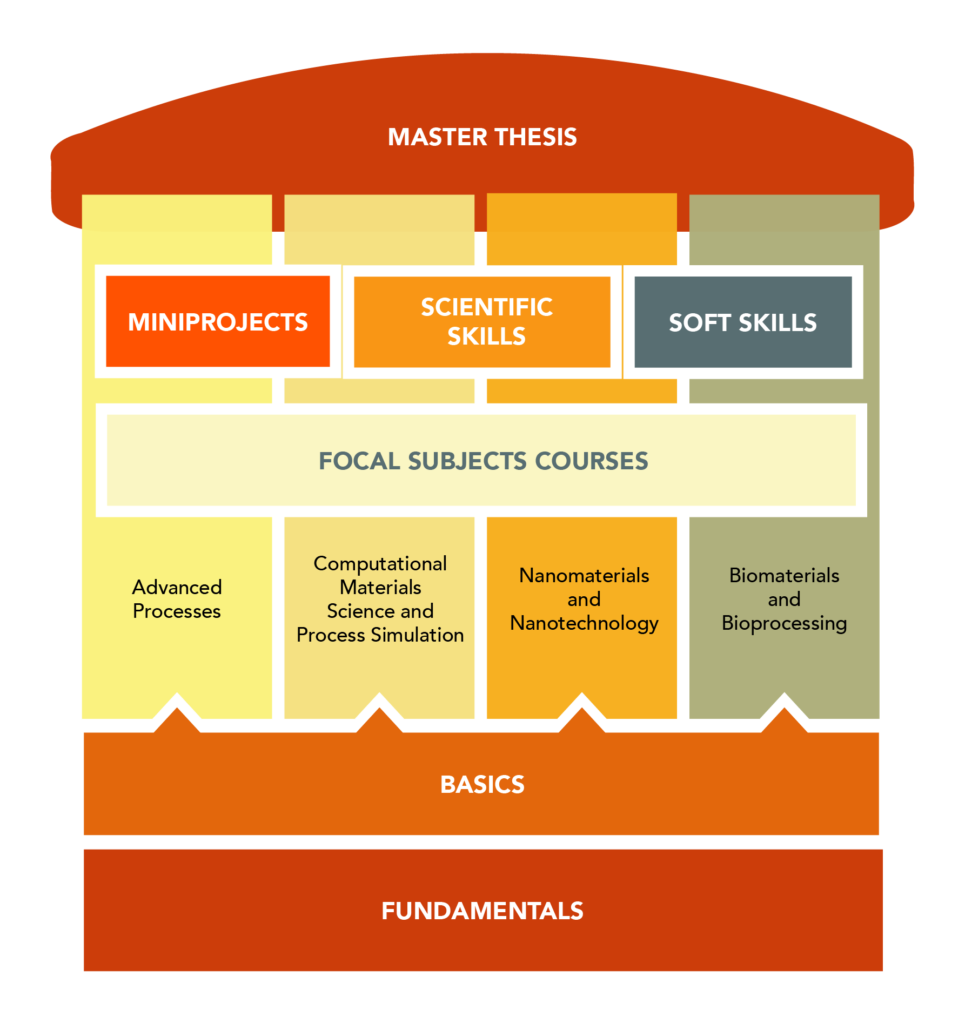
\includegraphics[width=0.5\textwidth]{map_structure}
	\caption{MAP program structure\cite{map_web}}
	\label{map_struct}
\end{figure}

Tables should be referenced in the same way as figures (though “Table” should always be written out in full). The table caption should be placed above the table.
 
To use pictures in \LaTeX \ you should first save your images to the folder \textit{images/}. If you want to use other directories, specify them in the \textit{main.tex} file in the \textbackslash graphicspath\{...\}.
 
You can easily create images and graphs with tikz. For example if you have the experimental data points don't hurry to create excel diagrams. Check out how the package pgfplots can be used to retrieve the data from csv files.


\section*{Acknowledgments}
Write a brief acknowledgment of your supervisor(s) and any other people or major resources (not your lab neighbour for lending you a pipette!) which contributed to your project.

       \bibliography{literature}
\end{document}
